\chapter{Log AS}

In his paper \cite{ismail2013stability}, Ismail presents
$Log_AS$ a class of \textit{many-sorted} languages that share a common core of logical symbols and differ in a signature of non-logical symbols. In what follows, we identify a sort $\sigma$ with
the set of symbols of sort $\sigma$.

A $Log_AS$ language is a set of terms partitioned into three base syntactic types, $\sigma_S , \sigma_T ,$
and $\sigma_i$. Intuitively,
\begin{itemize}
  \item $\sigma_S$ is the set of terms denoting states
  \item $\sigma_T$ is the set of terms denoting time points
  \item $\sigma_I$ is the set of terms denoting anything else.
\end{itemize}

\section{Syntax}

An alphabet for $Log_A S$ consists of two sets of symbols: syncategorematic punctuation symbols and denoting symbols from a set $\sigma$ of syntactic types. The set $\sigma$ includes four types, including one for function symbols that produce a term of a certain type based on a single argument of a base type.

$Log_A S$ is a first-order language because the first argument of function symbols is restricted to base types. A $Log_A S$ alphabet is a union of four sets, including a signature set of symbols with designated syntactic types, a set of variables, a set of syncategorematic symbols, and a set of logical symbols.

The variables set is countably infinite and consists of variables with designated types from $\sigma$. The syncategorematic symbols set includes punctuation symbols such as brackets and parentheses, as well as the universal quantifier symbol $\forall$. The logical symbols set is the union of several sets of logical symbols.

\begin{enumerate}
  \item $\neg \in \sigma_S \to \sigma_S$
  \item $\{\land, \lor \} \subseteq \sigma_S \to \sigma_S \to \sigma_S$
  \item $\textsc{HoldsAt} \in \sigma_S \to \sigma_T \to \sigma_S$
  \item $\prec \in \sigma_T \to \sigma_T \to \sigma_S$
\end{enumerate}

A $Log_AS$ language with signature $\Omega$ is denoted by $L_{\Omega}$ It
is the smallest set of terms formed according to the following
rules, where $\tau$ and $\tau_i (i \in \mathbb{N})$ are terms in $L_{\Omega}$

\begin{itemize}
  \item $\Xi \subset L_{\Omega}$
  \item $c \in L_{\Omega}$, where $c \in \Omega$ is a constant symbol.
  \item $f(\tau_1, \tau_2, \dots, \tau_n) \in L_{\Omega}$, where $f \in \Omega$ is of type
        $\varsigma_1 \dots \to \varsigma_n \to \varsigma  (n > 0)$ and $\tau_i$ is of type of $\varsigma_i$.
  \item $\neg \tau \in L_{\Omega}$, where $\tau \in \sigma_S$.
  \item $(\tau_1 \otimes \tau_2) \in L_{\Omega}$, where $\otimes \in \{\land, \lor\}$ and $\tau_1, \tau_2 \in \sigma_S$.
  \item $\forall x(\tau) \in L_{\Omega}$, where $x \in \Xi$ and $\tau \in \sigma_S$.
  \item $\textsc{HoldsAt}(\tau_1, \tau_2) \in L_{\Omega}$, where $\tau_1 \in \sigma_S$ and $\tau_2 \in \sigma_T$.
  \item $\prec(\tau_1, \tau_2) \in L_{\Omega}$, where $\tau_1, \tau_2 \in \sigma_T$.
\end{itemize}


\section{Semantics}

\begin{defn} $A  \ Log_AS$ structure is a \textit{quadruple} $\mathfrak{S}$
  = $\langle \mathcal{D}, \mathfrak{A}, \mathfrak{h}, < \rangle$ where
\end{defn}

\begin{itemize}
  \item $\mathcal{D}$, the domain of discourse, is a set with two disjoint, non-
        empty, countable subsets $\mathcal{S}  \ and\  \mathcal{T}$.
  \item $\mathfrak{A} = \langle \mathcal{S}, +, \cdot, -, \bot, \top \rangle $ is a
        complete Boolean algebra.
  \item $\mathfrak{h} : \mathcal{S} \times \mathcal{T} \to \mathcal{S}$ satisfies the following properties,
        for every $\hat{\mathcal{S}} \subseteq \mathcal{S}, s \in \mathcal{S}$ and $t, t_1, t_2 \in \mathcal{T}$:
        \begin{enumerate}
          \item $\mathfrak{h}(-s, t)= -  \mathfrak{h}(s, t)$.
          \item $\displaystyle \mathfrak{h}(\prod_{s\in \hat{\mathcal{S}}} s, t) = \prod_{s\in \hat{\mathcal{S}}} \mathfrak{h}(s, t)$.
          \item $\mathfrak{h}(\mathfrak{h}(s, t_1), t_2) = \mathfrak{h}(s, t_1)$.
          \item If $\displaystyle \prod_{t \in \mathcal{T}} \mathfrak{h}(s, t)= \top, \ then \ s = \top$.
        \end{enumerate}
  \item $< : \mathcal{T} \times \mathcal{T} \to \mathcal{S}$ defines an irreflexive linear order on $\mathcal{T}$ which is serial in both
        directors that is, $<$ is constrained as follows, for every distinct $t_1, t_2, t_3 \in \mathcal{T}$:
        \begin{enumerate}
          \item $t_1 < t_2 = - (t_2 < t_1)$.
          \item $[(t_1 < t_2) \cdot (t_2 < t_3)] + t_1 < t_3 = t_1 < t_3$.
          \item $t_1 < t_1 = \bot$.
          \item $\sum_{t \in \mathcal{T}} t < t_1 = \sum_{t \in \mathcal{T}} t_1 < t = \top$.
        \end{enumerate}
  \item For $t_1, t_2, t_3 \in \mathcal{T}, \mathfrak{h}(t_1 < t_2, t_3) = t_1 < t_2$.
\end{itemize}

\begin{defn}
  A \textit{valuation} $\mathcal{V}$ for a $Log_AS$ language $L_{\Omega}$ is a triple $\langle \mathfrak{S}, \mathcal{V}_{\Omega}, \mathcal{V}_{\Xi} \rangle$ where
\end{defn}
\begin{itemize}
  \item $\mathfrak{S} = \langle \mathcal{D}, \mathfrak{A}, \mathfrak{h}, < \rangle$ is a $Log_AS$ structure.
  \item $\mathcal{V}_{\Omega}$ is a function that assigns to each constant of sort $\varsigma$ in $\Omega$ an element of $\mathcal{D}_{\varsigma}$.
        and to each function symbol $f \in \Omega$ of sort $\varsigma_1 \to \cdots \to \varsigma_n \to \varsigma$ an
        n-adic function $\mathcal{V}_{\Omega}(f) :  \times_{i=1} \mathcal{D}_{\varsigma_i} \to \mathcal{D}_{\varsigma}$; and
  \item $\mathcal{V}_{\Xi} : \Xi \to \mathcal{D}$ is a function (called the \textit{variable assignment}) where
        for every $x \in \Xi$ if $s \in \mathcal{S}$ then $v_{\Xi} \in \mathcal{D}_{\varsigma}$.
\end{itemize}

for a valuation $\mathcal{V} = \langle \mathfrak{S}, \mathcal{V}_{\Omega}, \mathcal{V}_{\Xi} \rangle$ with
$x \in \Xi$ of sort $\varsigma$ and $a \in \mathcal{D}_{\varsigma}$, $\mathcal{V}[x/a] = \langle \mathfrak{S}, \mathcal{V}_{\Omega}, \mathcal{V}_{\Xi}[a/x] \rangle$
where $\mathcal{V}_{\Xi}[a/x](x) = a$, and $\mathcal{V}_{\Xi}[a/x](y) = \mathcal{V}_{\Xi}(y)$ for $y \in \Xi$ with $y \neq x$.

\begin{defn}
  Let $L_{\Omega}$ be a $Log_AS$ language and $\mathcal{V}$ be a valuation for $L_{\Omega}$. An interpretation of the terms of $L_{\Omega}$ given by a function
  \textlbrackdbl .\textrbrackdbl$^{\mathcal{V}}$:
\end{defn}
\begin{itemize}
  \item $\llbracket x \rrbracket^{\mathcal{V}} = \mathcal{V}_{\Xi}(x)$ for $x \in \Xi$ a variable symbol.
  \item $\llbracket c \rrbracket^{\mathcal{V}} = \mathcal{V}_{\Omega}(c)$ for $c \in \Omega$ a constant symbol.
  \item $\llbracket f(\tau_1, \cdots, \tau_n) \rrbracket^{\mathcal{V}} = \mathcal{V}_{\Omega}(f)(\llbracket \tau_1 \rrbracket^{\mathcal{V}}, \cdots, \llbracket\tau_n \rrbracket^{\mathcal{V}})$,
        for an n-adic $(n \geq 1)$ function symbol $f \in \Omega$
  \item $\llbracket \tau_1 \land \tau_2 \rrbracket^{\mathcal{V}} = \llbracket \tau_1 \rrbracket^{\mathcal{V}} \cdot \llbracket \tau_2 \rrbracket^{\mathcal{V}}$.
  \item $\llbracket \tau_1 \lor \tau_2 \rrbracket^{\mathcal{V}} = \llbracket \tau_1 \rrbracket^{\mathcal{V}} + \llbracket \tau_2 \rrbracket^{\mathcal{V}}$.
  \item $\llbracket \neg \tau \rrbracket^{\mathcal{V}} = - \llbracket \tau \rrbracket^{\mathcal{V}}$.
  \item $\llbracket \forall x(\tau) \rrbracket^{\mathcal{V}} = \prod_{a \in \mathcal{D}_{\varsigma}} \llbracket \tau \rrbracket^{\mathcal{V}[a/x]}$. where $x$ is of sort $\varsigma$
  \item $\llbracket \textsc{HoldsAt}(\tau_1, \tau_2)\rrbracket^{\mathcal{V}} = \mathfrak{h}(\llbracket \tau_1 \rrbracket^{\mathcal{V}}, \llbracket \tau_2 \rrbracket^{\mathcal{V}})$.
  \item $\llbracket (\tau_1 \prec \tau_2) \rrbracket^{\mathcal{V}} = \llbracket \tau_1 \rrbracket^{\mathcal{V}} < \llbracket \tau_2 \rrbracket^{\mathcal{V}}$.
\end{itemize}

\begin{defn}
  Let $L_{\Omega}$ be a $Log_AS$ language.
  For every $\phi \in \sigma_S$ and $\Gamma \subseteq \sigma_S, \phi$ is a \textit{logical consequence} of $\Gamma$ (written $\Gamma \models \phi$) if for every $L_{\Omega}$ valuation $\mathcal{V}$,
  $\displaystyle \prod_{\gamma \in \Gamma} \llbracket \gamma \rrbracket^{\mathcal{V}} \leq \llbracket \phi \rrbracket^{\mathcal{V}}$.

\end{defn}

\section{Stability}
Ismail \cite{ismail2013stability} classifies states based on the \textit{temporal stability}, Temporal stability refers to the tendency, or
lack thereof, of a state to change from holding to not holding, and the general patterns of such changes.
Three main types of states are \textit{eternal}, \textit{permanent}, and \textit{temporary}.

\subsection{Eternal States}
Eternal states are those that never start or end, and they either always hold or never hold.
These types of states are the most stable over time, and sentences that represent them are the least likely to change in meaning.
\begin{figure}[H]
  \centering
  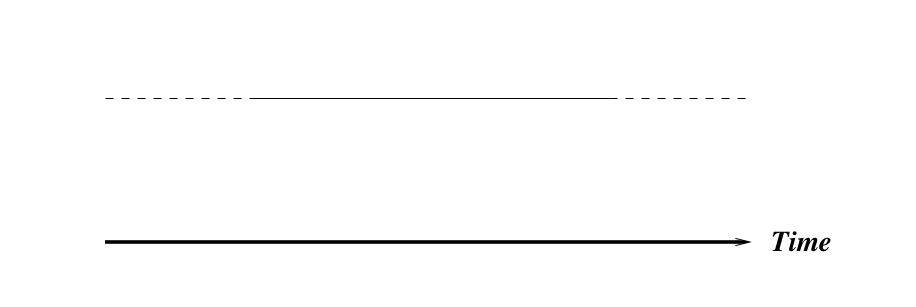
\includegraphics[width=0.7\textwidth]{images/eternal-states.png}
  \caption{An eternally holding state}
  \label{fig:eternal}
\end{figure}

The following sentences are examples of eternal states.

\begin{enumerate}
  \item Whales are fish.\footnote{A state’s being eternal has nothing to do with its actually holding, even though whales are not fish,
          this represents an eternal states. If someone believes that whales re fish and later comes to believe that they are actually mammals, only one thing would have
          changed, namely the believer’s state of mind. Whales did not become mammals; rather, the person
          would assume that they were and shall always be mammals.\cite{ismail2001reasoning}}
  \item God exists.
  \item John's birthday is on the 21st of March.
\end{enumerate}

\begin{defn}
  $s \in \mathcal{S}$ is an \textit{eternal} if $\displaystyle \sum_{t \in \mathcal{T}} \mathfrak{h}(s, t) \leq \prod_{t \in \mathcal{T}} \mathfrak{h}(s, t)$.
\end{defn}

\textsc{Eter} denotes the set of eternal states.

\subsubsection{Atemporal States}
\begin{defn}
  $s \in \mathcal{S}$ is \textit{atemporal} if $\mathfrak{h}(s, t) = s$ for every $t \in \mathcal{T}$.
\end{defn}
\textsc{Atemp} denotes the set of atemporal states.
\subsection{Permanent States}
Permanent states differ from eternal states in that they may start to hold at some point.
Once a permanent state begins, it will continue to hold indefinitely. The \textit{Onset} mentioned here refers to the event of the permanent state starting to hold.


\begin{figure}[H]
  \centering
  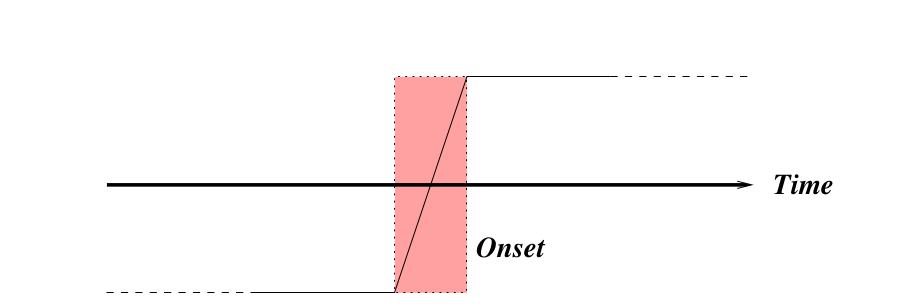
\includegraphics[width=0.7\textwidth]{images/permanent-states.png}
  \caption{A permanent state}
  \label{fig:permanent}
\end{figure}

The following sentences are examples of permanent states.


\begin{enumerate}
  \item John has died.
  \item John had turned 22.\footnote{There's a claim that the perfect aspect/tense always signals a permanent state a permanent states is the perfect}
  \item I had my bachelor degree.
\end{enumerate}

\begin{defn}
  A state $s \in \mathcal{S}$ is \textit{permanent} if
  \begin{enumerate}
    \item $s \neq \bot$,
    \item $\displaystyle \prod_{t \in \mathcal{T}} \mathfrak{h}(s, t) = \bot$ and
    \item for every, $t_1, t_2 \in \mathcal{T}, [\mathfrak{h(s, t_1)} \cdot (t_1 < t_2)] \leq \mathfrak{h(s, t_2)}$.
  \end{enumerate}
\end{defn}

\textsc{Perm} demotes the set of permanent states.

\subsubsection{CO permanent States}
Let $\textsc{Co-Perm}$ denote the set of complements of states in \textsc{Perm}.

A state $s \in \textsc{Co-Perm}$ if and only if
\begin{enumerate}
  \item $s \neq \top$,
  \item $\displaystyle \prod_{t \in \mathcal{T}} \mathfrak{h}(s, t) = \top$ and
  \item for every, $t_1, t_2 \in \mathcal{T}, [\mathfrak{h}(s, t_1) \cdot (t_2 < t_1)] \leq \mathfrak{h}(s, t_2)$.
\end{enumerate}


\subsection{Temporary States}
A \textit{temporary state} may repetitively start to hold and cease to hold. Unlike
permanent states, temporary states do not just have an onset; they have both an onset and a cessation.
These are events that mark the state starting to hold and ceasing to hold, respectively. For every time
the state holds, there shall be a unique onset-cessation pair.

\begin{figure}[H]
  \centering
  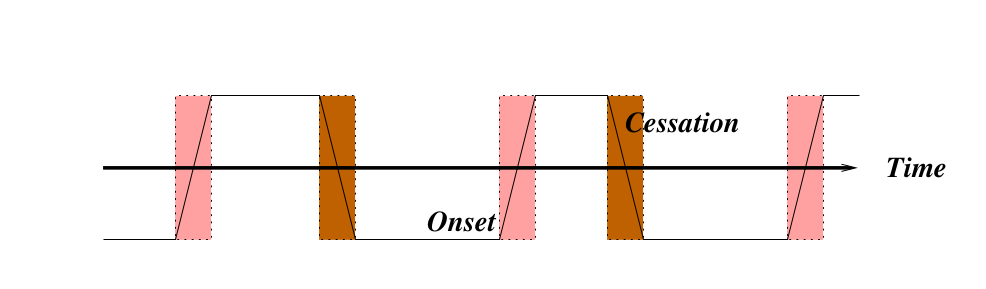
\includegraphics[width=0.7\textwidth]{images/temp-states.png}
  \caption{A temporary state}
  \label{fig:temporary}
\end{figure}

The following sentences are examples of temporary states.

\begin{itemize}
  \item I am crossing the street.
\end{itemize}

Temporary states are totally unconstrained and may, thus,
contingently exhibit patterns of holding similar to those of \textsc{Eter}, \textsc{Perm}, and \textsc{CO-Perm}. However, some states strictly
resist the anti-temporary patterns. For example, the state of
an event being in progress is a temporary state which will
never hold eternally, permanently, or co-permanently, since
an event necessarily starts and ends.

\subsubsection{Transient States}

\begin{defn}
  A state $s$ is \textit{transient} if
  \begin{enumerate}
    \item $\displaystyle \sum_{t_1 \in \mathcal{T}} \sum_{t_2 \in \mathcal{T}} [(t_1 < t_2) \cdot \mathfrak{h}(s, t_1) \cdot - \mathfrak{h}(s, t_2)] = \top$ and
    \item $\displaystyle \sum_{t_1 \in \mathcal{T}} \sum_{t_2 \in \mathcal{T}} [(t_2 < t_1) \cdot \mathfrak{h}(s, t_1) \cdot - \mathfrak{h}(s, t_2)] = \top$.
  \end{enumerate}
\end{defn}

\textsc{Trans} denotes the set of transient states.


$\textsc{Trans} \subseteq \textsc{Temp}$



\begin{figure}[H]
  \centering
  \caption{Venn diagram of the stability sets}

  \tikzset{every picture/.style={line width=0.75pt}} %set default line width to 0.75pt        


  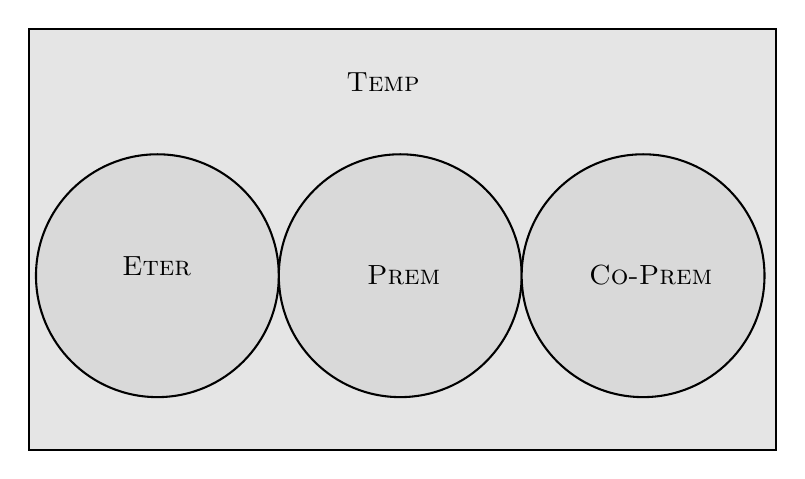
\begin{tikzpicture}[x=0.75pt,y=0.75pt,yscale=-1,xscale=1]
    %uncomment if require: \path (0,310); %set diagram left start at 0, and has height of 310

    %Shape: Rectangle [id:dp9438939353832179] 
    \draw  [fill=gray!20] (64.5,13.5) -- (424.5,13.5) -- (424.5,216.5) -- (64.5,216.5) -- cycle ;
    %Shape: Circle [id:dp6623230466810723] 
    \draw  [fill=gray!30] (68,132.5) .. controls (68,100.19) and (94.19,74) .. (126.5,74) .. controls (158.81,74) and (185,100.19) .. (185,132.5) .. controls (185,164.81) and (158.81,191) .. (126.5,191) .. controls (94.19,191) and (68,164.81) .. (68,132.5) -- cycle ;
    %Shape: Circle [id:dp16392927570144655] 
    \draw  [fill=gray!30] (185,132.5) .. controls (185,100.19) and (211.19,74) .. (243.5,74) .. controls (275.81,74) and (302,100.19) .. (302,132.5) .. controls (302,164.81) and (275.81,191) .. (243.5,191) .. controls (211.19,191) and (185,164.81) .. (185,132.5) -- cycle ;
    %Shape: Circle [id:dp6100961383336985] 
    \draw  [fill=gray!30] (302,132.5) .. controls (302,100.19) and (328.19,74) .. (360.5,74) .. controls (392.81,74) and (419,100.19) .. (419,132.5) .. controls (419,164.81) and (392.81,191) .. (360.5,191) .. controls (328.19,191) and (302,164.81) .. (302,132.5) -- cycle ;

    % Text Node
    \draw (108,122) node [anchor=north west][inner sep=0.75pt]   [align=center] {\textsc{Eter}};
    % Text Node
    \draw (226,126) node [anchor=north west][inner sep=0.75pt]   [align=center] {\textsc{Prem}};
    % Text Node
    \draw (333,126) node [anchor=north west][inner sep=0.75pt]   [align=center] {\textsc{Co-Prem}};
    % Text Node
    \draw (216,33) node [anchor=north west][inner sep=0.75pt]   [align=center] {\textsc{Temp}};


  \end{tikzpicture}
  \label{fig:venn}
\end{figure}

